%% FEUP THESIS STYLE for LaTeX2e
%% how to use feupteses (English version)
%%
%% FEUP, JCL & JCF, 31 July 2012
%%
%% PLEASE send improvements to jlopes at fe.up.pt and to jcf at fe.up.pt
%%

%%========================================
%% Commands: pdflatex tese
%%           bibtex tese
%%           makeindex tese (only if creating an index) 
%%           pdflatex tese
%% Alternative
%%          latexmk -pdf tese.tex
%%========================================

\documentclass[11pt,a4paper,oneside,openright]{report}

%% For iso-8859-1 (latin1), comment next line and uncomment the second line
\usepackage[utf8]{inputenc}
%\usepackage[greek,english]{babel}
%\usepackage[latin1]{inputenc}
\usepackage{amsmath}

\usepackage{listings}

%% English version

%% MIEEC options
%%\usepackage[mieec]{feupteses}
%\usepackage[mieec,juri]{feupteses}
\usepackage[mieec,final]{feupteses}
\usepackage{float}
\usepackage{geometry}
\geometry{left=2.5cm,right=2.5cm,top=2.5cm,bottom=2.5cm}
\usepackage{graphicx}
\usepackage{subfig}
\usepackage{multirow}
\usepackage{algorithm}
\usepackage{algpseudocode}

%% Additional options for feupteses.sty:
%% - onpaper: links are not shown (for paper versions)
%% - backrefs: include back references from bibliography to citation  place

%% Uncomment to create an index (at the end of the document)
%\makeindex

%% Path to the figures directory
%% TIP: use folder ``figures'' to keep all your figures
\graphicspath{{figures/}}

%%----------------------------------------
%% TIP: if you want to define more macros, use an external file to keep them
%some macro definitions

% format
\newcommand{\class}[1]{{\normalfont\slshape #1\/}}

% entities
\newcommand{\Feup}{Faculdade de Engenharia da Universidade do Porto}

\newcommand{\svg}{\class{SVG}}
\newcommand{\scada}{\class{SCADA}}
\newcommand{\scadadms}{\class{SCADA/DMS}}


%%----------------------------------------

%%========================================
%% Start of document
%%========================================
\begin{document}
\nocite{*}


%%----------------------------------------
%% Information about the work
%%----------------------------------------
\title{API design and implementation of a management interface for SDN whitebox switches}

\author{Rubens Jesus Alves Figueiredo}

%% Uncomment next line for date of submission
\thesisdate{\today}

%% Comment next line copyright text if not used
%%\copyrightnotice{Vânia Filomena Madureira Vieira, 2017}

\supervisor{Supervisor}{Ana Cristina Costa Aguiar}

%% Uncomment next line if necessary
\supervisor{External Supervisor}{Dr. Hagen Woesner}

%% Uncomment committee stuff in the final version if used
%\committeetext{Approved by \ldots:}
%\committeemember{President}{Name of the President}
%\committeemember{Referee}{Name of the Referee}
%\committeemember{Referee}{Name of the Referee}
%\signature

%% Specify cover logo (in folder ``figures'')
\logo{uporto-feup.pdf}

%% Uncomment next line for additional text  below the author's name (front page)
%%\additionalfronttext{
%%    \textbf{Final Report} \\
%%    Preparação da Dissertação
%%}

%%----------------------------------------
%% Preliminary materials
%%----------------------------------------

\begin{Prolog}
    \chapter*{Resumo}
%\addcontentsline{toc}{chapter}{Resumo}
Os requisitos crescentes dos serviços em nuvem de hoje requerem a evolução da infraestrutura de rede para suportar a quantidade crescente de dados que são
processados todos os dias. Isso significa que os operadores de rede de centros de dados devem projectar ou adaptar os seus ambientes de rede em nuvem para fornecer
uma conexão estável e confiável.  Uma infraestrutura otimizada muitas vezes significa também, a redução de custos na utilização da rede e na economia de energia.

\par À medida que as redes crescem e são mais complexas, os sistemas devem ser implantados que permitem acompanhar de perto os recursos que compõem a rede, 
enquanto também permitindo uma certa liberdade para a possível mudança constante da rede. Como tal, as soluções típicas dos fornecedores não se encaixam realmente
nessa paisagem de constante mudança, uma vez que apresentam soluções muito sólidas e verticalmente integradas. O paradigma do Software Defined Networking, no entanto,
é capaz de resolver esse problema, pois permite o controlo centralizado das redes subjacentes, proporcionando visibilidade e controlo sobre os dispositivos da
rede, simplificando o diagnóstico de erros e a solução de problemas.

\par Neste trabalho, propomos um sistema de gerenciamento modular para controladores de rede definidas por Software ds centros de dados da nuvem, fornecendo aos
administradores de sistemas um plataforma simples para visualização da topologia de rede, monitorizar portas de dispositivos de rede, etc. A modularidade também 
fornece uma plataforma simples para estender a funcionalidade dos controladores de rede, que podem ser usados para implementar a detecção de anormalidades de rede e
optimizar os caminhos de encaminhamento de fluxo, entre outros.

\chapter*{Abstract}
%\addcontentsline{toc}{chapter}{Abstract}
%\https://www.th-wildau.de/fileadmin/dokumente/studiengaenge/europaeisches_management/dokumente/Dokumente_EM_Ba/Abstracts_in_English.pdf

The rising requirements of today's cloud services require the evolution of networking infrastructure to support the increasing amount of data that is processed
every day. This means that data center network operators must design or adapt their cloud networking environments to provide a stable and reliable connection.
Better optimized infrastructure often also means cost reductions in network utilization and energy savings.

\par As networks grow larger and more complex, systems must be put in place that allow for closely monitoring the resources that make up the network, while also 
allowing for a certain freedom for the possible constant change of the network. As such, typical vendor solutions don't really fit into this ever changing landscape,
since they present very solid and vertically integrated solutions. The Software Defined Networking paradigm, however, is able to solve this issue, since it enables
the centralized control of the underlying networks, providing visibility and control over the network's devices, simplifying error diagnosis and troubleshooting. 

\par In this work we propose a modular management system for cloud data center Software Defined Networking controllers, providing system administrators a simple
platform to view their network's topology, monitor networking devices ports, etc. The modularity also provides a simple platform to extend the functionality 
of the networking controllers, that can be used to implement detection of network abnormalities and optimize flow forwarding paths, among others.
 % the abstract
    %\chapter*{Acknowledgments}
%\addcontentsline{toc}{chapter}{Agradecimentos}

First of all, I'd like to thank my supervisor Dr. Ana Aguiar, for the constant support and guidance that was provided. I'd would also like to thank for the 
opportunity of finishing my master's thesis in a foreign company, and spending these past few months in Germany was an amazing experience.

\par The constant environment of teaching and support provided by Dr. Hagen Woesner and the team at BISDN was undoubtedly a big factor in my adjustment in Germany.
The experience I gained, both technically and personally was a big mark during the development of this thesis, and the working atmosphere contributed immensely
for my integration there.

\par Next I would like to thank my parents and brother, for the immense support that they showed during my time abroad, and the understanding that only they could
provide during these past few years. 

\par Finally, a certain group of people who helped me grow during these years in university could not be forgot.
  % the acknowledgments
    % \cleardoublepage
\thispagestyle{plain}

\vspace*{8cm}

\begin{flushright}
   \textsl{``By the time you've sorted out a complicated idea
   \\into little steps that even a stupid machine can deal with,
    \\you’ve certainly learned something about it yourself.}\\
\vspace*{1.5cm}
           Douglas Adams
\end{flushright}
    % initial quotation if desired
    % \cleardoublepage
    \pdfbookmark[0]{Contents}{contents}
    \tableofcontents
    \cleardoublepage
    \pdfbookmark[0]{List of Figures}{figures}
    \listoffigures
    \cleardoublepage
    \pdfbookmark[0]{List of Tables}{tables}
    \listoftables
    \chapter*{Abreviaturas e Símbolos}
%\addcontentsline{toc}{chapter}{Abbreviations}
\chaptermark{ABREVIATURAS E SÍMBOLOS}
\usepackage[utf8]{inputenc}
\begin{flushleft}
\begin{tabular}{l p{0.8\linewidth}}
EM       & Electromagnetic\\
\end{tabular}
\end{flushleft}

  % the list of abbreviations used
\end{Prolog}

%%----------------------------------------
%% Body
%%----------------------------------------
\StartBody

%% TIP: use a separate file for each chapter
../doc/chapters/introduction.tex 
%\inclcude{chapters/background}
/home/rubinhus/feup/tese/doc/chapters/sdn.tex
\chapter{Network Management} \label{chap:nm} %% chapter 3

\par This chapter focuses on the management of networks, where we explore what is most necessary to obtain a comprehensive understanding of the network; formalize the statistics that can be reported via OpenFlow; see some 
research that has been done in the management of SDN applications, including what existing controllers provide us; and finally explore the way that DDoS detection and mitigation is usually implemented.

\section {Introduction}

\par As networks grow larger and more complex, systems must be put in place that allow for closely monitoring the resources that make up the network, while also allowing for a certain freedom for the possible constant change of the 
network. As such, typical vendor solutions don't really fit into this ever changing landscape, since they present very solid and vertically integrated solutions. The SDN paradigm, however, is able to solve this issue, since it 
enables for the centralized control of the underlying networks, which provides visibility and even control over the network, simplifying network diagnosis or troubleshooting. 
\par Although SDN is a promising paradigm in terms of networking management, it also introduces some points of failure that are non existing, or not as impactful in current networking deployments. This is related, for example,
to the centralization of the controller, which makes it susceptible to Denial-of-Service attacks or even the possibility of some malicious attacker that could possibly exploit the privileged view that the SDN controller has.
\par The topic of network management is very extensive, due to the several components that make up today's networks, and the vast amount of information that they provide. It can be summed up as the operation and maintenance 
of network infrastructure so that the service it provides is not only "healthy", but also is operated at a level that keeps costs down for service providers. 

\section {Requirements for management systems}

\par As the complexity of the networks, and network devices that compose them grow bigger and bigger, the management systems should accommodate for the their necessities. As such, the basic groups of requirements for management 
functions are that defined in the ITU-T X 700 Recommendation \cite {CITE - ITU T Recomendation} are:

\begin {itemize}
    \item \textbf {Fault management} is the capability for detection, isolation and correction of abnormal operation in the system
    \item \textbf {Accounting management} provides ways to monitor the system resource utilization, and using this data to generate information about the costs that the operation of a certain resource will incur. This 
        allows for better optimizing the network utilization of network, as it provides insights on how to plan the evolution of the network
    \item \textbf {Configuration management} is related to the maintenance and updates of hardware and software in the network, and the general setup of devices that allow to start, maintain and terminate services 
    \item \textbf {Performance management} relates to monitor systems for the traffic utilization, response time, performance and logging histories. This allows to maintain Service Level Agreements (SLA) from the service
        provider and the client, providing better services even in cases of unusual traffic.
    \item \textbf {Security management} enables setting up security policies in terms of access control to resources, private information protection, among others.
\end {itemize}


\par A network management system usually consists of a centralized station, and management agents running on the network devices. Using management protocols, the agents can report to the station information about the its operational 
status, which includes information ranging from CPU load to bandwith usage. Typically this information can be retrieved by the controller polling the agents, or the agents sending information on their own, usually to inform
status changes. Using this information, the network operator can get insight on the performance or possible errors of the devices that are monitored. In the next section, we explore one of the most popular management protocols,
SNMP.

\section {SNMP}

The Simple Network Management Protocol is an IETF defined protocol that allows for the interconnection of networking devices, and provide a structured way to retrieve relevant information about these devices. As the name suggests,
SNMP allows for a simplified approach to network monitoring, since it reduces the complexity of the functions that the management agent needs to comply with, which bring several advantages, like reducing
the costs for development of management tools; provides a way to monitor, independently from different hardware providers the resources; and also supports freedom in extending the protocol in order to include other aspects of 
network operation. \cite{CITE - RFC 1157} %% XXX cite https://tools.ietf.org/html/rfc1157
\par  The architectural model of SNMP can be described in figure \ref{fig:snmp}.
    
\begin{figure} [!htbp]
    \centering
    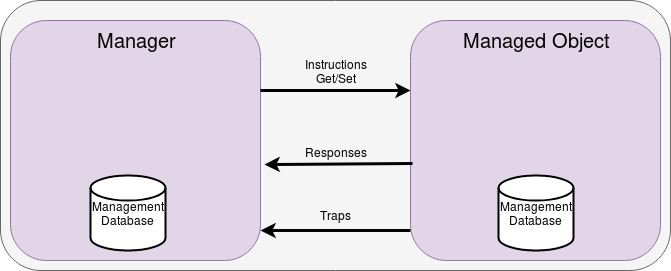
\includegraphics[width=.6\textwidth]{nm/snmp_arch}
    \caption{Architectural components of SNMP}
    \label{fig:snmp}
\end{figure}

The management database is one of the most important components of this system, because it serves as a reference to the entities that are managed in the SNMP protocol. The formal name for this database is the MIB - Management 
Information Base \cite {CITE - RFC 1155}, and its composed of a collection of objects.

\par Each object has a name, syntax and encoding \cite {CITE - RFC 1156}. The name of the object, more specifically, the \textit {Object Identifier (OID)}, is a reference to the object itself. This name is usually a 
list of integers, and they serve to build a tree-like hierarchy. This structure allows for the organization of all objects in a logical pattern, as there is a parent node, that contains references to their children, 
that provide different indexes for different objects. For human readability, there is usually a \textit {Object Descriptor}, to refer to the object type. The syntax defines the type of data structure in the object type; and 
the encoding describes how the object type is transmitted on the network. In the context of this thesis, an important group is the interfaces group, as this exposes information about the interfaces present in a system. It's OID 
is the .3.6.1.2.1.2., and contains the number of interfaces in a system, and a table containing the counters related to the interface status, like the received unicast packets, the physical address, among others. The flexibility of
the MIB allows for vendors to introduce their own databases into the MIB, while also remaining compatible with the standardized one.

\par Due to its permanence in the market, the protocol has suffered some large changes since its original design. SNMPv3 now supports important changes to the original one, most notably in the security aspects, introducing strong
authentication and encryption capabilities.

\section {Data Center Networks (DCN)}

\par The rising demand of services like music and video streaming, or mass data storage, brings an increase of demand of compute and storage infrastructures, and the shift to the cloud computing model has led to a
proliferation of large data-centers, containing thousands of physical nodes. Related to this growth is the focus on moving not only servers to a virtualised environment, by having one physical host several virtual machines and
client applications, but moving also the networking functions to a virtual environment, by replacing the dedicated network hardware with generic compute resources, in a paradigm called \textit{Network Function Virtualisation (NFV)} 
\cite {CITE - OPENSDWN}. One of the bigger gains of using NFV, is the possibility of separation of each virtual network (VN), which guarantees better performance isolation and application of Quality of Service (QoS) rules
\cite {CITE - Data center virtualisation a survey}. 
\par The design of the network architecture is central to the data-center networks, as the placement for physical hosts and virtual machines allows for sharing the resources and create a logical hierarchy of network devices. The 
study on the design of DCN has resulted in the creation of typical DC topologies, like fat-tree topologies (as seen in \ref {nm/fattree}), or others, including de Bruijn server only networks, or BCube switch heavy networks 
\cite{ popa_cost_2010 }. This approach allows for the traffic characteristics, resource consumption and costs of the networking devices be understood, so that causes for failure of this network are understood and mitigated, 
and the entire DC can run on the most optimal possible way. The organization in the DCN also allows for traffic in the network being resistant to failure scenarios, since there are multiple paths that can redirect packets 
to the correct destination, even if a link to a switch fails.

\begin{figure} [!htbp]
    \centering
    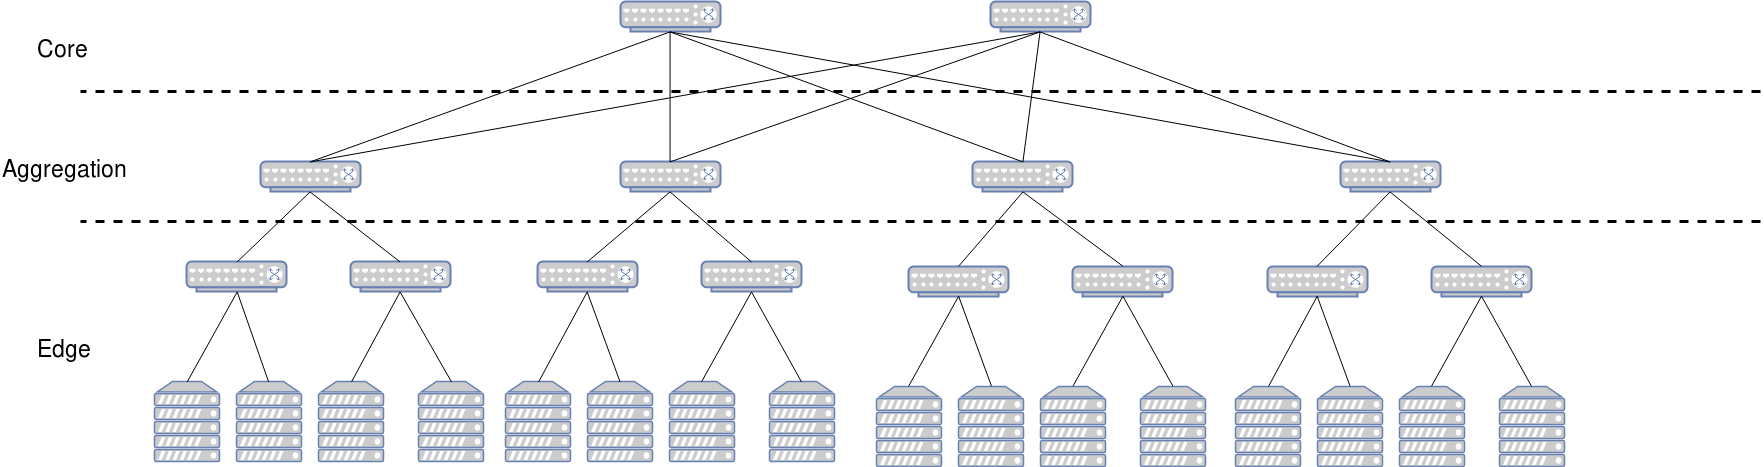
\includegraphics[width=1\textwidth]{nm/fattree}
    \caption{Visual representation of the fat tree topology commonly used in data centers}
    \label{nm/fattree}
\end{figure}

\subsection {DCN Traffic}

\par So that solutions for network management in data-centers can be developed, first there needs to an understanding of the traffic characteristics and resource allocation, and utilize this information to shape the DC fabric.
The several studies proposed in traffic engineering for traditional networks do need to be revised in DCN's, since metrics like propagation delay, can be negligible, due to the physical proximity of nodes in DC's 
\cite{CITE - data_center_virt_survey}. However, studies on DCN's have proven difficult, since many data-center operators do not wish to publish information about their applications and services. Also contributing to this fact is
the impossibility of separating the different classes of data centers, since deployments across campus, private and cloud data-centers serve different purposes and have different applications.
\par By collecting data from different types of DC's, several studies have been made about the traffic characteristics \cite{ CITE - dc_networks_chars, CITE - dc_traffic_chars, CITE - fb_datacenter}:

\begin {itemize}
    \item The placement of VMs and servers effects the bandwidth and link capacity, due to the variety of applications that can be running on the servers at any time, and this non-uniform placement of VMs contributes to higher
        amounts of traffic originating from the same rack
    \item The majority of flows \footnote {flows are usually defined as} are described as being small in size, and short in duration, which are usually described as \textit {mice} flows. The counterpart to these are the 
        \textit {elephant} flows, which occupy a very large share of the bandwidth, and degrade application performance, due to choking effect to the latency-sensitive mice flows. Applications are tied to the type of traffic they
        generate, where online gaming, VoIP and multimedia broadcasting usually originate mice flows, where the large data transfers and file-sharing originate in elephant flows. However, these flows which account for 80\% of 
        total traffic only occur less than 10\% of total flows \cite {CITE - Broadcom Engineered Elephant flow for boosting ... }.
    \item In a normal situation, link utilization is low in the layers apart from the core switches. In addition to this discovery, losses are associated with spikes in traffic, instead being related to high utilization 
        of the link, which is one of the effects of the previously mentioned elephant flows.
\end {itemize}

\subsection {Limitations}

\subsection {DCN and SDN}

\par The centralized view that SDN controllers maintain over the networks allows for it to keep the information about the flows currently present in the network. As such, in the SDN paradigm, there is possibility to flexibly control 
the path that the packets take in the network, and improve performance of the network at a large scale. By joining the information available on DCN and SDN, the requirements for traffic engineering (TE) in SDN, from
the perspective of flow control are flow management, fault tolerance and traffic analysis \cite { CITE - traffic_engineering_sdn}. This set of four requirements set the base for properly monitoring a DCN from the 
perspective of the SDN paradigm.
\par The next section are taken from \cite { CITE - traffic_engineering_sdn}.

\subsubsection {Flow management}

Flow management refers to the capability that the controller has to set rules for packet forwarding, and maintain the low overhead that is associated with registering a new flow mod, and also limiting the amount of flow entries, 
as hardware switches usually have a set amount of flow entries that it can support. Further in this document, we explore the effect that the amount of flow entries has on OVS, where increasing the amount of flow entries also 
increases the packet loss between two hosts.
\par If we consider the fat-tree topology, then one obvious result is the fact that if one controller is responsible for the management of the entire underlying topology, then one possible results is the creation of one bottleneck
when the rules need to be deployed to a node. When the switch receives a new packet, and there are no rules to properly forward this packet, then the packet is redirected to the controller, on the form of a \textsc{PACKET\_IN} 
message, and after processing this packet a new flow mod is sent to the switch. The problem with this scenario lies in the delay that it takes between the reception of the packet, and the installation of the new
flow entry, which can be a contributing factor in packet losses in the data plane. This is an attack vector that is also explored in Distributed Denial of Service (DDoS) attacks for SDN platforms, as in an extreme scenario,
the spoofed packet addresses will not have matches on the tables, which then result on overflowing the controller \cite {early_detection_sdn_ddos}.
\par A solution for this issue is then related to decreasing the number of messages sent to the controller, by introducing some load balancing concepts. One of these concepts is related to the way that we can install the flow 
entries on the switch. The information present in the packets serve to generate the flow-match entries that are deployed on the table. To reduce the number of interactions between the controller and OF switches, then we can 
reduce the number of match fields present in the flow mods, which reduces the number of flow entries on the switch and the controller messages. Another solution is related to distribute the controller among the network, 
but keeping them connected via a separate channel.

\subsubsection {Fault tolerance}

Although the switches are connected in a way that are able to mitigate link, or other switch failures, in the case of faults occurring there needs to be the possibility of creation of new forwarding rules. An even bigger 
concern lies in the case when the controller fails, which will pose a larger problem in the network. For the case of node failure, fast recovery means that the OF controller can reactively react on link failures, by signaling the
switches to forward packets toward new locations; or proactively, by setting the rules prior to the occurrence of the failure. In the case that the failure is short lived, then the controller is also responsible of resetting the 
paths to the optimal state.
\par In the case of controller failover, then the backup controllers should act on this failure, and act as the new master. OF switches should connect to the set of available controllers, which should coordinate the management of 
the switch amongst themselves. After the switches first connection to the controllers, they should maintain this connection alive, but the controllers have the possibility of changing their roles. The controller roles are as follows:

\begin {itemize}
    \item \textsc {OFPCD\_ROLE\_EQUAL}, where the controller has full access to the switch, receiving all incoming messages, and can modify the state of the switch
    \item \textsc {OFPCD\_ROLE\_MASTER}, which is a similar status to the previous one, but where the switch ensures that only one switch is connected as the master role
    \item \textsc {OFPCD\_ROLE\_SLAVE} is a role that controllers has read-only access to the switch, having no permissions for altering the state of the switch. The only message that controllers registered with this role receive
        are the port-status messages
\end {itemize}

As previously mentioned, the way that controllers handle their connection is independent of the OpenFlow connection, and the failover should occur with minimal changes to the underlying flow rules and overhead.

\subsubsection {Traffic analysis}

So that the management tools can correctly display information about the state of the network, status statistics should be continuously collected and analysed. These statistics should provide the information about flows, packets
and ports, so that the measured metrics can serve as a baseline for the decisions of the controller to adapt the flow mods to enable the best possible performance. For the statistics collection there are two possible ways of 
getting the data: by continuously sampling packets from the switches; or applying sampling techniques, and generalizing the information from the sampled data \cite{CITE - low_overhead_te_elephants_detec}. The problem here lies
in the collection of the statistics in poses a problem for large scale deployments, where continuously polling the network devices introduces both overhead and very large amounts of data to be parsed, or the data is not enough
to detect failures in a short amount of time.

\section {Statistics}

\subsection {OpenFlow}

After exploring the requirements for network management, and the way the SDN model can support developing better systems, we now focus on the possibilites for obtaining this information from the networking devices. The OpenFlow 
protocol maintains a set of counters for each flow entry, port and group statistics, and this information can be queried to obtain a general view on the status of each OF switch. By sending specific controller-to-switch messages,
the switch will return a set of the maintained statistics, which can then be parsed and analysed further. 
\par Sending the port statistics message returns an array with the measured counters for each port. These counters include information like the amount of received and transmitted bytes/ packets, errors and dropped packets, and the
duration that the port is alive. 
\par The next important message is the \textsc{OFMP\_FLOW} message, since this allows for getting the individual flow statistics, and obtain the information about each flow entry, including the time that it has been set on the switch,
the number of packets/bytes in the flow, and the match fields. Also worth noting are the aggregate flow messages which describe how many packets are in the total flow entries, and also the number of flow entries that exist.
\par Also relevant is the information that is retrieved using the group statistics, as they allow to monitor the number of flows that direct to the group, and again the packet/ byte count that are matched with this group.
\par As we can see, the information provided from these messages allows for a comprehensive view of the state of each switch, and a network management system (NMS) should utilize this information to achieve an understading of the 
state of the network. One problem arises, however, when the periodic requests generate too much information, and the control channel is overflowed with messages of port statistics, which is a possible scenario when the
flow tables start getting too large. As such, a different alternative is to sample a small amount of packets from the switch, send the packet headers to the controller. One popular standard for applying this technique is 
\textit{sFlow}, and is described in the next section.

\subsection {sFlow}



\chapter {Berlin Institute for Software Defined Networks} \label{chap:bisdn} %% chapter 3

\section {Introduction}

\begin{figure} [!htbp]
    \centering
    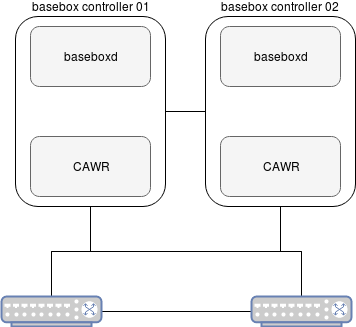
\includegraphics[width=.4\textwidth]{bisdn/basebox}
    \caption{Basebox architecture}
\end{figure}

As the SDN market grows larger and larger in the networking world, new applications and products are developed and improved. Seeing the prevalence of closed source and proprietary solutions for this market, a need for open
products that enable further growth and innovation in cloud DCNs is evident. The main gain in moving from vertically integrated solutions, is the decrease of costs involved, as cheaper solutions can be found in whitebox 
\footnote {whitebox switches are} switches and open sourced networking applications. With this motivation, BISDN developed Basebox, a Linux-powered solution to integrate switches and SDN controllers, allowing for data center 
operators to configure and manage networks using linux commands, removing the need for having to manage several devices with different interfaces and workflows, and adding the capability of running standard networking applications 
on top of the controllers and switches. Basebox also includes the possiblity of running in a failover scenario, by introducing a backup controller for the network, and the possibility of creating a giant switch abstraction, 
by adding another controller, CAWR, and having this manage all the southbound switches.

\par In this chapter we focus on this product, on the first two sections some characteristics of the developed product are described, then we focus on the development of a management API, presenting the required technologies that 
were implemented, and then finally display the results that were obtained in this part of the thesis.

\section {Existing product}

\subsection {baseboxd}
\subsection {CAWR}

\section {Management API}

Due to the capabilities of Basebox of being a SDN controller used in data centers and a mission critical component for the network operators, it needed management capabilities, so that managing and operating infrastructure becomes 
an easier task. As such, the original problem presented was to build an interface extending the original work, so that the network statistics and the information of the topology could be easily displayed. There were several steps
then necessary to understand the problem, and be able to choose the best approach to this problem. The requirements for the proposed system were:

\begin {itemize}
    \item Display the topology information reported by CAWR, including the internal switch links, and the LACP discovered bond interfaces on the servers
    \item Display the port and link statistics for both switches
    \item Design an alerting system, so that network operators can be informed of changes on the network state
    \item Provide some diagnostic capabilities
\end {itemize}

\par The development of the work was the divided on two parts: the first part would be to implement the API needed to export the port statistics from baseboxd and CAWR, including a Graphical User Interface (GUI); and the second 
part was to study the alerting system, that would look into the statistics provided by the controllers, and design some rules so that QoS rules could be applied in the final product. This section describes the technologies needed 
to implement the API for Basebox.

\subsection {Data models}

Data models are abstract concepts that map the properties of entities and organizes their data, also defining how they relate to each other. To create a switch management interface, the entities we want to model are then 
the switches themselves, with attributes like the switch name, and the port counters, and the relationships of the data will allow us to display the links and topology of the network. One of the considerations that were taken into 
account when choosing the data models was the compatibility with standardized data models by the organizational entities like the IETF and the OpenConfig. 
\par The \textit{ NETCONF } network configuration model, which we explore further in \ref{ssec:netconf} also defines a data modelling language known as \textit{ YANG }, which is used in this protocol to model its configuration 
and data,and the remote procedure calls \cite { CITE - rfc 6020 }. By utilizing models defined in this language, the following condition is met: since this is a specific language for configuration and monitoring of networking 
devices, the existing data models will be similar to the ones that should be employed in the development of the management API. YANG data model defines the hierarchy of data between a NETCONF client and server with the objective
of smooth integration with the existing system's infrastructure. 
\par The systems we aim to model with these requirements are then two: the topology between the servers and switches, and the port statistics for each port one the switch. Since there is no data model that would accurately describe
both of them correctly, for the topology we chose the IETF network data model \footnote {https://github.com/YangModels/yang/blob/master/experimental/ietf-extracted-YANG-modules/ietf-network\%402017-12-13.yang}, and the 
OpenConfig interfaces data model \footnote {https://github.com/openconfig/public/tree/1040d11c089c74084c64c234bee3691ec70e8a9f/release/models/interfaces}, which contains the counters for each port.

\subsubsection {Topology}

The topology data model maps a collection of nodes, and the relationships between each node, called a link. This also allows for describing the network in a vertical hierarchy, by displaying relationships between several layers,
which can then be used to display the entire networking stack, for example displaying the physical links between nodes, their connections at layer 2 and layer 3 of the OSI model, and the virtualised relationships that the elements 
could have in a cloud deployement. As the development of the product continues, and more features are added, for example, layer 3 routing, then we require a flexible data model that can be extended to support the new capabilities.

\begin{figure} [!htbp]
    \centering
    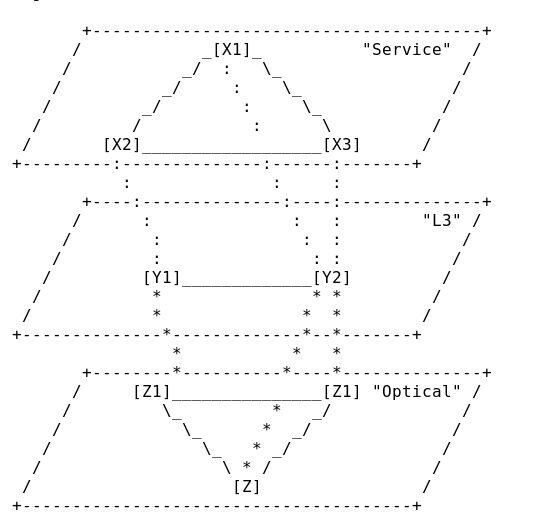
\includegraphics[width=.3\textwidth]{bisdn/network_stack_topologies}
    \caption{Topology hierarchy achievable with this example \cite {CITE - https://www.ietf.org/id/draft-ietf-i2rs-yang-network-topo-20.txt}}
\end{figure}

\par Mapping the data model to the real world data is then adding the two types of information the data model expects: the first one composed of adding the different networks that composed the entire topology, including their
nodes and network types; and then using the previous information to build the links between each of the nodes, using the termination points the model exposes. In the implementation of the management API there was no need to implement 
underlying networks, but the extensibility this provides will be useful in the future.
\par Displaying the topology proved useful for CAWR, which provides the big switch topology, since this controller is directly connected to the underlying switches, and can see the links among these networking devices. The connection
to the bonded interface on the servers can also be monitored, since these can be configured to use LACP messages to report their status. To display the links between the switches, the information that LLDP provides is used, 
and if the controller is extended to be able to use LLDP to the servers, the further information can be filled into this data model, and provide a richer view on the status of each server.

\begin{figure} [h]
    \begin{subfigure}
    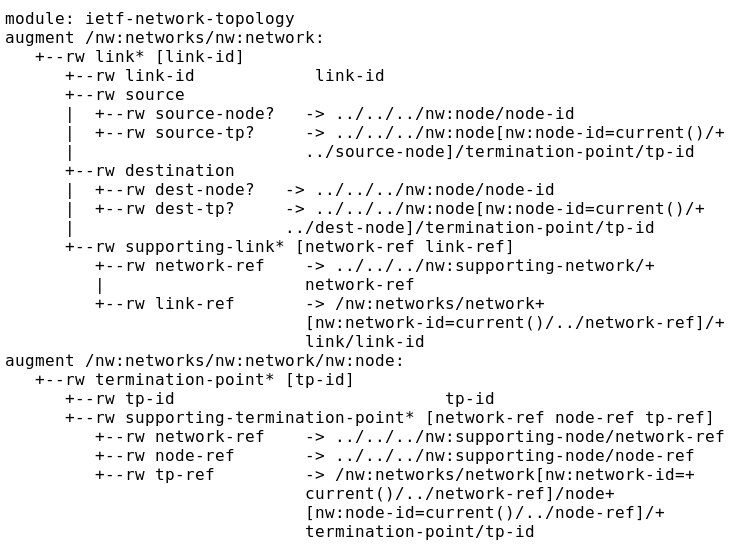
\includegraphics[width=0.5\textwidth]{bisdn/ietf_link}
    \end{subfigure}
    \begin{subfigure}
    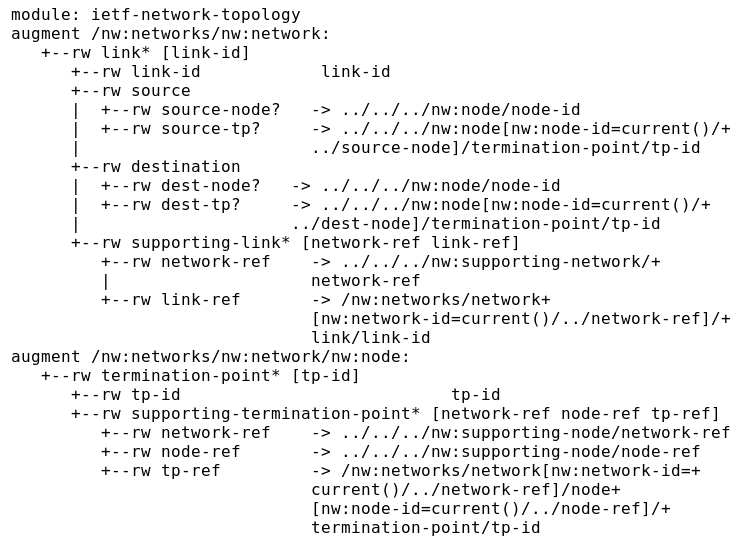
\includegraphics[width=0.5\textwidth]{bisdn/ietf_node}
    \end{subfigure}
\caption{The IETF description for the nodes and links in the draft proposal for network topologies \cite {CITE - https://www.ietf.org/id/draft-ietf-i2rs-yang-network-topo-20.txt} }
\end{figure}

\subsubsection {Port statistics}

\par Modelling the port statistics to build a management interface requires first understanding of the OpenFlow statistics. As previously mentioned, OF switches maintain a set of counters, similar to SNMP, that provide information 
about the state of the ports, group, flow and table stats. The statistics that are exposed from OF are the following:

\begin{table}[]
    \centering
    \caption{OpenFlow port statistics}
    \label{my-label}
    \begin{tabular}{l | l || l | l}
       uint64\_t & rx\_packets     & uint64\_t & tx\_packets;     \\ \hline
       uint64\_t & rx\_bytes;      & uint64\_t & tx\_bytes;       \\ \hline
       uint64\_t & rx\_bytes;      & uint64\_t & tx\_dropped;     \\ \hline
       uint64\_t & rx\_errors;     & uint64\_t & tx\_errors;      \\ \hline
       uint64\_t & rx\_frame\_err; & uint64\_t & tx\_over\_err;   \\ \hline
       uint64\_t & rx\_crc\_err;   &                              \\ \hline
       uint64\_t & collisions;     &                              \\ \hline
       uint32\_t & duration\_sec;  &                              \\ \hline
       uint32\_t & duration\_nsec; &                 
    \end{tabular}
\end{table}

\par The chosen data model should then accurately model the fields that we need to expose, and the data type of counters we wish to measure. In this case, the prevalence of other controllers allows to use the same data models present 
in their implementations. OpenConfig \footnote{http://www.openconfig.net/} maintains a set of vendor neutral data models, written in YANG, allowing network operators to use standardized models for their networking infrastructure.
The entire set of published models can be accessed in their github page \footnote {https://github.com/openconfig/public}.

\subsection {Protocols}

None of the controllers had a clear way of obtaining the statistics apart from manually looking in the terminal and following the logs exposed and waiting for the appropriate output. There needs to be then a controllable, to export
this information and displaying them in a clear way. The solution was to develop a Graphical User Interface (GUI) for easily displaying the live statistics from the server, however there still was the problem of having to 
define the API that build the transport channel between baseboxd and CAWR to the GUI server. In this section we describe the two \textit {Remote Procedure Call (RPC)} systems that were researched, and focus on the advantages which
led to the final decision of implementing gRPC on Basebox.

\subsubsection {NETCONF} \label {ssec:netconf}

Despite it's dominance on network management products, SNMP features some bad characteristics that pose an obstacle for the widespread use in network configuration, and not only network management, like 
\cite {CITE - https://tools.ietf.org/html/rfc3535}: 

\begin {itemize}
    \item Incompleteness of the devices features
    \item SNMP access can sometimes crash systems, or return wrong data
    \item Unavailability of MIB modules, which forces users to use CLI's
    \item Poor performance 
    \item Security is difficult to handle
\end {itemize}

\par The IETF then, in light of this feedback obtained from network operators, started developing a protocol that allowed for the installation, manipulation and deletion of configuration of networking devices called NETCONF, which 
enables devices to expose a full API to their systems. This protocol, based in client/ server communication and is based in the four layers, as can be seen in the following image:

\begin{figure} [!htbp]
    \centering
    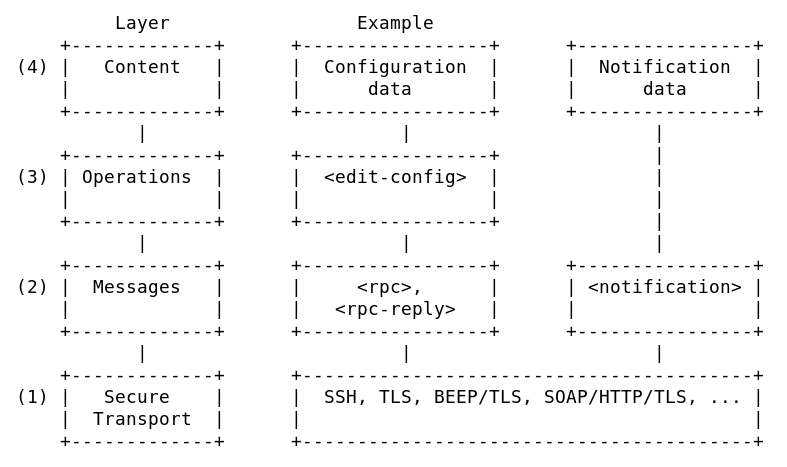
\includegraphics[width=.4\textwidth]{bisdn/netconf}
    \caption{NETCONF protocol layers \cite {CITE - Basebox architecture}}
\end{figure}

\par Data models and operations, covered in detail in the previous section, is related to the Content layer on the image, so this will not be covered in this section. 
\par Configuration of a network device can be complex, and managing separate configurations between device startup and normal operation is a difficult task, but there is occasional need for this capability. NETCONF defines the 
existence of different \textit{datastores} to enable this feature, allowing the network operator to set an initial configuration, used when the device is initialized, and switching to the running datastore when the device is ready
to maintain normal operation. This concept of datastores also enables the creation of a candidate datastore, providing the capability of testing configurations on the network device, checking for any possible errors, while making
sure that there is no impact on the current configuration of the device. After the changes have been tested and validated, a <commit> operation can be used to deploy the new configuration to the running datastore.
\par Another useful feature that is described in the NETCONF protocol, is the possibility of using the rollback-on-error capability. When rolling a new change, and if the system is enabled to support this feature,
NETCONF can detect errors in the changes done to the configurations, and return the system to the previous state that is error free. 
\par The NETCONF API provides several operations to interact with the managed devices to get system information and push new configurations. The set of supported operations in the base NETCONF protocol can be accessed in 
\url{https://tools.ietf.org/html/rfc6241#section-7}. 
\par In regards to the transport layer, NETCONF is able to run on top of several protocols. However, NETCONF requires that a persistent connection is maintained between devices, and this connection should be reliable, and support
transmission failure. In addition, the security should be handled by the transport layer \cite { CITE - https://www.ietf.org/slides/slides-edu-netconf-yang-00.pdf}, providing the guarantee that transactions are done in a 
cryptographically secure channel, between two authenticated hosts. As a results, typical NETCONF implementations are based on SSH or TLS protocols.

\subsubsection {gRPC}  \label {ssec:grpc}

The basic idea behind the RPC system is defining services by setting the interaction between remote systems, allowing for directly calling objects on remote systems. Based in the client/server communications 
pattern, gRPC allows for interactions between different environments, even implemented with different programming languages, all based on the same data structure. This data structure can be serialized using another modelling 
language, called \textit {protobuf}, which will define the data, which is defined as messages, and the services that contain the RPC calls between systems. Since this system is based on the HTTP2 transport layer, we are able to
use the advantages that this protocol provides us.
\par Despite the serialization language used in gRPC is based on protocol buffers, unlike YANG, there are some projects \footnote {https://github.com/openconfig/goyang} that enable the translation between YANG to protofile,
which allows us to use the data models we chose, only adding one extra step to convert the files.
\par Despite both protocols capability of meeting the requirements that were presented to us, the gRPC framework was chosen due to several reasons:

\begin {itemize}
    \item Both frameworks allow us to use the standardized data models currently proposed by the IETF and OpenConfig
    \item NETCONF trades information as XML encoded information, for both the edit and get config operations; while gRPC allows to handle information in a way that’s native to the language implementation of the client/server
    \item The integration with the existing system was easier: since gRPC has implementations for the languages that the controllers are developed on (i.e. C++/ Python), this framework was easier to implement 
        than NETCONF, which would have required integration with third party tools, or a longer development cycle to make sure that the developed applications would met the requirements
\end {itemize}

\section {Results}


\chapter{Statistical Detection} \label{chap:stat_det} %% chapter 3

As a result of the large scale of current data centers, maintaining control over these networks proves a difficult task. Networks operators must then adapt to the current situation by improving the monitoring infrastructures 
to allow faster response to problems.  Building a feature complete management API for a SDN controller means that information obtained from the port and flow statistics previously implemented should return information 
about the global state of the network, so that root-cause analysis of the source of network issues can be done faster and easier, which reflect on better service and lower costs for network operators. 
\par Network behaviour analysis is defined by the constant monitoring of a network, so that events that compromise the "healthy" state of the network can be removed or mitigated. These include not only cases where the anomalies are
caused with malicious intent, like the case of DDoS attacks, but also failure of network devices or changes in user behaviour \cite {traffic_anomaly_control_charts}. These systems are equipped with alarm capabilities, so that 
system administrators can quickly respond to changes, possibly even giving some information about the source of the problem. However, the automation of these monitoring processes means that the possible existence
of false alarms reduces the operators capabilities to act on actual failures. 
\par This chapter focuses on the recent research done in order to implement systems that rely on statistical analysis for monitoring the state of the networks and detection of abnormalities.

\section {Elephant flow detection}

Detection of network anomalies is subject to intense research, and as such, several methods were developed, that assume different levels of control over the network and provide different results to different applications. Our goal
in this section is then to provide a description of the different types of network issues that can occur, and some proposed solutions for these issues.
\par The problem of detection of traffic anomalies has been subject to extensive research, and several different approaches have been proposed. These methods are based on different techniques 
\cite {http://shiftleft.com/mirrors/www.hpl.hp.com/personal/Praveen_Yalagandula/papers/INFOCOM11.pdf}:

\begin {itemize}
    \item Modifications to the applications and services to notify the controller about the state of the traffic on each service. Despite this approach resulting in the most accurate "detection" of network anomalies, the support 
for this technique is not extensive, due to the required changes to each service, and it does not account for abrupt changes on the traffic
    \item By setting hard limits on the transmission capabilities of each port and switch, the controller is ensured of the non existence of flows that could impact network performance. This is a mitigation strategy that
does not scale well to very large networks, since it requires the storage of the rules imposed to every port, and can potentially lead to the inefficient use of network resources, reducing flexibly on the DCN's.
    \item By employing sampling and collection techniques, using mechanisms like sFlow \ref{subsec:sflow}, and building the profiles of the normal state of the network, this method can detect outliers that deviate from the
normal state of the network. Utilizing this method reduces impact that continuously polling the network might have, while reducing impact on the packet and byte counts 
\cite {https://www.cert.org/flocon/2006/presentations/packet_sample_anomoly2006.pdf}, but the loss of information inherent to sampling may be a challenge on successful deployment, which should account for optimal sampling 
strategies and inference from the obtained statistics.
    \item Periodic polling of the statistics from the switch, and employing statistical analysis methods to determine change points in the state of the network.
\end {itemize}

\section {Time series analysis}

Understanding processes and their results is a key factor in the success of implementing new features, or analysing existing ones for their efficiency and output. This analysis, important for the different fields in engineering,
economics, health, allows obtaining information about the normal and abnormal state of each underlying process, provide forecasts and predictions on short and long term behaviour of the relevant data, classify and cluster 
information, and more. The act of collecting and processing the data, over a period of time is called \textit{time series analysis}. 
\par Monitoring systems provide a guarantee in quality engineering, since they allow to follow a system and its properties, and notify operators if changes happen that impact the normal status of a relevant parameter. These changes
can be occasional or systematic, but should the state of the system deviate from the limits set by the operators, researching the cause of the errors can reveal some errors or malfunctions in the system. \textit{Change detection}
is the study of the different parameters of the system, and determining the points where these cause a significant deviation from the normal operation. In network traffic analysis, these methods can be applied to determine when 
the behaviour of certain flows, that can be monitored over metrics originating from the controller and switches, impact the traffic characteristics. One key part on the application of changepoint detection is the understanding 
and selection of the proper metrics to monitor, to ensure that these are sensitive to the traffic changes. One other important consideration in applying changepoint detection mechanisms is the reduction of false alarms, that occur 
when the metrics are too sensitive to traffic changes, and limit the network operators capability of accurately responding to real network issues. 
\par Change detection mechanisms are classified as follow \cite { CITE -https://www.net.in.tum.de/fileadmin/TUM/NET/NET-2010-06-1.pdf#cite.feinstein03}:

\begin {itemize}
    \item One of the most important distinctions in change detection theory is the difference between online and offline detection. Offline, or batch detection methods consider a fixed length of observations, and retrospectively 
analyse the dataset to determine the time where the change, or changes took place. Online detection, or sequential detection, unlike batch detection which uses all the available observations to detect the changes, including the
ones obtained after the change took place, is based on the determination of the change points based on the arrival of the new data, allowing for determining the change as fast as possible.
\cite { CITE - http://citeseerx.ist.psu.edu/viewdoc/download?doi=10.1.1.425.1477&rep=rep1&type=pdf}. 
    % TODO - Bayesian change detection
    \item An important criteria for the classification of changepoint detection algorithms is the knowledge of the distribution that the system has before the change occurs. A Bayesian system considers the 
    \item Finally, the last important distinction is related to the scalability, and relate to the amount of data that needs to be stored to accurately implement detection on new samples. Parametric approaches rely on learning a 
probability distribution from the monitored variables, and using this learned data to estimate the unknown parameters, after which the training data can be discarded. Non-parametric models however, do not take into consideration the
distribution of the monitored variables, and analyse statistical properties instead. The cost of this analysis is that the previous data must be stored to provide better results, but this problem can be mitigated using 
algorithms using sliding window or moving averages.
\end {itemize}

\subsection {Mathematical formulations}

A time series can be defined as a stream of observations $X = \{x_1, ... x_i\}$, where $x_i$ is a vector arriving at time $i$. The time series $X$ can also be described as the sum of the following components: $S_t$,
which refers to the seasonal component of the data; $T_t$, which defines the trend of the data, and $R_t$ represents the residual values, accounting for non expected variation and noise.

\begin {equation*}
\centering
y_t = S_t + T_t + R_t
\end {equation*}

Or:

\begin {equation*}
\centering
y_t = S_t * T_t * R_t
\end {equation*}

\par In regards to the classification of the trends according to the type of change, they can be classified as:

\begin {itemize}
  \item \textbf {Deterministic} when the trend consistently increase/decrease
  \item \textbf {Stochastic} when the opposite happens
\end {itemize}

\par Approximating the time series data to a model allows for generating predictions for the next values, since the relationship between two variables in the data is then known. The Box-Jenkins method defines the steps of building the model as \cite{Box, 
G.E.P. 
and 
J.M. 
Jenkins, 
1976, 
Time 
series 
analysis: 
Forecasting 
and 
control 
(Holden-Day, 
San 
Francisco, 
CA). }:

\begin {enumerate}
  \item \textbf{Identification}
  \item \textbf{Fitting}
  \item \textbf{Checking}
\end {enumerate}

The most common models present in trends are:

\begin{table}[h]
\centering
\label{tab:trends}
\begin{tabular}{|c|c|}
\hline
Linear      & $y = m \cdot x + b$ \\ \hline
Polynomial  & $y = b + c_1 \cdot x + \dotso + c_n \cdot x^n$  \\ \hline
Exponential & $y = c \cdot  x^b$     \\ \hline
Logarithmic & $y = a \cdot ln(x) + b$        \\ \hline
\end{tabular}
\caption{Trend models}
\end{table}

\par Time series data usually present a non stationary behaviour, that are characterized by changes in the mean and variance. Statistical methods require, however, stationarity in the data. The presence of trends and cyclic behaviours
is the most common violation of stationary, and can be removed through differencing.

\begin {equation*}
\centering
\nabla X_t = X_t - X_{t-1} = (1-B)X_t
\end {equation*}

Where,

\begin {equation*}
\centering
B X_t = X_{t-1}
\end {equation*}

\subsection {Forecasting}

Under the assumption that the underlying process can be modeled by previous historical values, and assuming this model remains true for future measurements, the time series data historical behaviour can be used to generate forecasts for future values
in the time series. 

\subsection {Change Detection}

 A relevant indicator for the
validity of the generated forecasts is the forecast error, that is calculated via the difference between the real measurements and the predicted value. Furthermore, by assuming a distribution for the forecast error, and a certain significance level, it is possible 
to validate the generated forecasts, and detect values that do not fit the model, accusing a possible variation in the parameters of the model. As such, the prediction error is able to be employed in change detection algorithms. This
prediction error can be defined as:

\begin {equation*}
\centering
\epsilon_t = x_t - \hat{x}_t
\end {equation*}

\subsection {Performance Evaluation}

\subsection {Control charts}

\chapter{Monitoring SDN Switches} \label{chap:mon_sdn} %% chapter 3

\section {Problem}

Developing solutions for use in mission critical environments requires the deep understanding and analysis of the requirements of these environments, like those
present in large data centers. The Basebox system (see section \ref{sec:bisdn}) is an example of these solutions, but lacks a system for monitoring and management 
of the network devices. Such a system should 

\begin {itemize}
    \item display the topology information reported by CAWR, including the internal switch links, and the LACP discovered bond interfaces on the servers,
    \item display the port and link statistics for both switches,
    \item design an alerting system, so that network operators can be informed of changes on the network state,
    \item provide diagnostic capabilities.
\end {itemize}

\par Also addressed by this system should be the definition of Quality-of-Service (QoS) policies, that maintains the levels of accepted traffic behaviour of each 
device in the network, and identifies and applies some automatic mitigation strategy when the system does not perform according to normal state. By understanding
data center traffic characteristics, one of the largest problems are the existence of \textit{elephant flows}, that impact the available bandwidth of the network.
As such, the development of a full management system should also include a system that receives the incoming port statistics, analyses these, and applies
statistical analysis to manage the impact caused by elephant flows.

\section {Solution}

\begin{figure} [h]
    \centering
    \includegraphics[width=0.5\textwidth]{proposed_work/proposed_system}
    \caption{High-level visual description of the proposed system} \label{fig:pro_sys}
\end{figure}

\par Following the previously presented requirements, the proposed system is present in figure \ref{fig:pro_sys}. First, we add an interface for the controllers that 
exposes management information like the network's topology, statistics, etc. After this, we build an \textbf{Operations Support System} (OSS) that provides the basis 
for the development of applications that monitor the state of the network, using the implemented API to obtain the relevant information. This system allows
further separation of roles in the network, in contrast to a system where the controller would gather the roles of managing and monitor the network's status, 
increasing the load on the controllers. Furthermore, this architecture increases the modularity of the components, enabling hot-swapping different modules, and
allows parallel development of different features in the monitoring and management stack.

\par We provide a proof-of-concept composed of two components: the first is a Graphical User Interface (GUI) providing an user friendly interface to display 
topology and statistics, and the second is an intelligent system enabling the detection of elephant flows. In this section we describe in a high level way the 
approaches for the development of this system.

\subsection {GUI}

The primary use case for this component is following the changes in the underlying topology, while also allowing the monitoring some aspects of the port statistics,
and as such, the links between switches and the hosts, and the association between the ports and the switches should be displayed. Performance wise, this system must
run as fast as possible, and the transmission of data must not interfere with the systems operation. 

\par In order to reduce the memory requirements of the platform, and decrease the time that it takes for drawing topology updates, a decision was made to not store 
state, which would increase the time it takes for topology updates, with queries to store and load data from these databases. This also removes complexity as the 
system grows, where storing information about links and switches would dramatically increase database size.

\par Motivated by compatibility with standardized systems, choosing the data model for representing the underlying system required the investigation of similar 
systems, and the RFCs, or similar standardized documents that exist. 

\subsection {Elephant Flow detection}

The second component of our system was developed for monitoring the system statistics, and displaying alerts when elephant flows are detected. For this end, we have
implemented an algorithm for the detection part. 

\par By monitoring traffic changes in the switches ports, the developed system aims to detect the presence of large flows based on the traffic statistics obtained
from the API. As we assume the tree topology in data centers, seen in figure \ref{fig:fattree}, the testing environment must be designed to monitor the lower layer
edge switches, connected directly to the physical hosts. By monitoring the ports on these switches, we detect changes in the reported traffic statistics via a
developed Python script.

\chapter {Management API}

Due to the capabilities of Basebox of being a SDN controller used in data centers and a mission critical component for the network operators, it needed management capabilities, so that managing and operating infrastructure becomes 
an easier task. As such, the original problem presented was to build an interface extending the original work, so that the network statistics and the information of the topology could be easily displayed. There were several steps
then necessary to understand the problem, and be able to choose the best approach to this problem. The requirements for the proposed system were:

\begin {itemize}
    \item Display the topology information reported by CAWR, including the internal switch links, and the LACP discovered bond interfaces on the servers
    \item Display the port and link statistics for both switches
    \item Design an alerting system, so that network operators can be informed of changes on the network state
    \item Provide some diagnostic capabilities
\end {itemize}

\par The development of the work was the divided on two parts: the first part would be to implement the API needed to export the port statistics from baseboxd and CAWR, including a Graphical User Interface (GUI); and the second 
part was to study the alerting system, that would look into the statistics provided by the controllers, and design some rules so that QoS rules could be applied in the final product. This section describes the technologies needed 
to implement the API for Basebox.

\section {Data models}

Data models are abstract concepts that map the properties of entities and organizes their data, also defining how they relate to each other. To create a switch management interface, the entities we want to model are then 
the switches themselves, with attributes like the switch name, and the port counters, and the relationships of the data will allow us to display the links and topology of the network. One of the considerations that were taken into 
account when choosing the data models was the compatibility with standardized data models by the organizational entities like the IETF and the OpenConfig. 
\par The \textit{ NETCONF } network configuration model, which we explore further in \ref{ssec:netconf} also defines a data modelling language known as \textit{ YANG }, which is used in this protocol to model its configuration 
and data,and the remote procedure calls \cite { CITE - rfc 6020 }. By utilizing models defined in this language, the following condition is met: since this is a specific language for configuration and monitoring of networking 
devices, the existing data models will be similar to the ones that should be employed in the development of the management API. YANG data model defines the hierarchy of data between a NETCONF client and server with the objective
of smooth integration with the existing system's infrastructure. 
\par The systems we aim to model with these requirements are then two: the topology between the servers and switches, and the port statistics for each port one the switch. Since there is no data model that would accurately describe
both of them correctly, for the topology we chose the IETF network data model \footnote {https://github.com/YangModels/yang/blob/master/experimental/ietf-extracted-YANG-modules/ietf-network\%402017-12-13.yang}, and the 
OpenConfig interfaces data model \footnote {https://github.com/openconfig/public/tree/1040d11c089c74084c64c234bee3691ec70e8a9f/release/models/interfaces}, which contains the counters for each port.

\subsection {Topology}

The topology data model maps a collection of nodes, and the relationships between each node, called a link. This also allows for describing the network in a vertical hierarchy, by displaying relationships between several layers,
which can then be used to display the entire networking stack, for example displaying the physical links between nodes, their connections at layer 2 and layer 3 of the OSI model, and the virtualised relationships that the elements 
could have in a cloud deployement. As the development of the product continues, and more features are added, for example, layer 3 routing, then we require a flexible data model that can be extended to support the new capabilities.

\begin{figure} [!htbp]
    \centering
    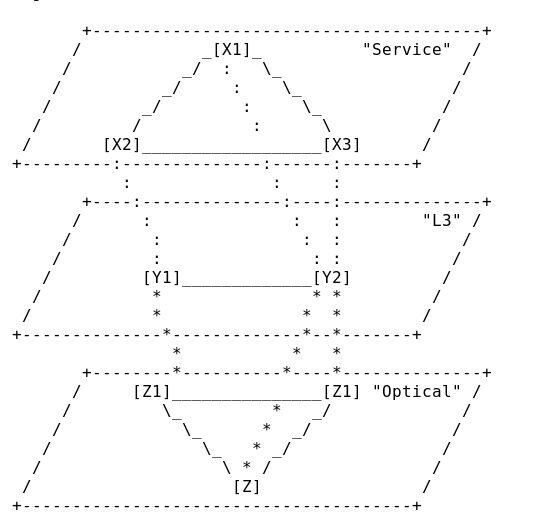
\includegraphics[width=.3\textwidth]{bisdn/network_stack_topologies}
    \caption{Topology hierarchy achievable with this example \cite {CITE - https://www.ietf.org/id/draft-ietf-i2rs-yang-network-topo-20.txt}}
\end{figure}

\par Mapping the data model to the real world data is then adding the two types of information the data model expects: the first one composed of adding the different networks that composed the entire topology, including their
nodes and network types; and then using the previous information to build the links between each of the nodes, using the termination points the model exposes. In the implementation of the management API there was no need to implement 
underlying networks, but the extensibility this provides will be useful in the future.
\par Displaying the topology proved useful for CAWR, which provides the big switch topology, since this controller is directly connected to the underlying switches, and can see the links among these networking devices. The connection
to the bonded interface on the servers can also be monitored, since these can be configured to use LACP messages to report their status. To display the links between the switches, the information that LLDP provides is used, 
and if the controller is extended to be able to use LLDP to the servers, the further information can be filled into this data model, and provide a richer view on the status of each server.

\begin{figure} [h]
    \begin{subfigure}
    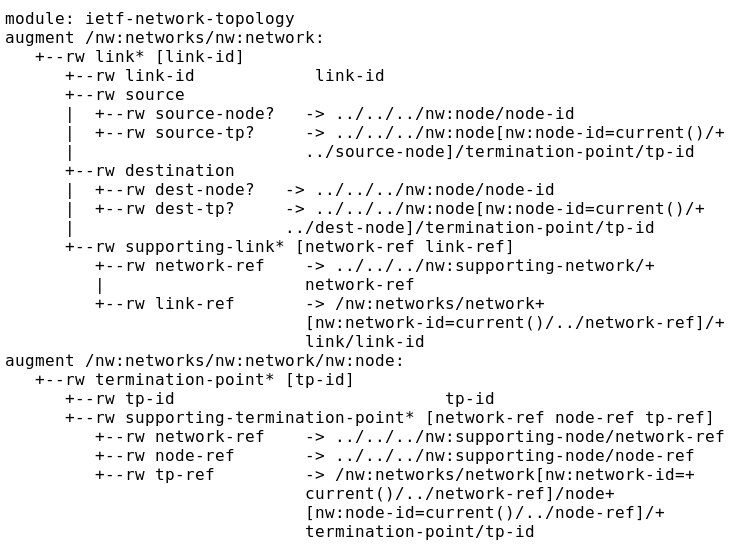
\includegraphics[width=0.5\textwidth]{bisdn/ietf_link}
    \end{subfigure}
    \begin{subfigure}
    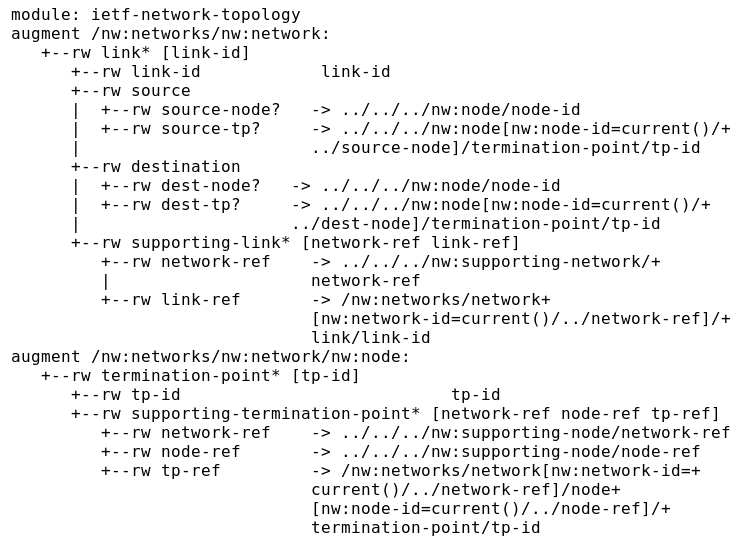
\includegraphics[width=0.5\textwidth]{bisdn/ietf_node}
    \end{subfigure}
\caption{The IETF description for the nodes and links in the draft proposal for network topologies \cite {CITE - https://www.ietf.org/id/draft-ietf-i2rs-yang-network-topo-20.txt} }
\end{figure}

\subsection {Port statistics}

\par Modelling the port statistics to build a management interface requires first understanding of the OpenFlow statistics. As previously mentioned, OF switches maintain a set of counters, similar to SNMP, that provide information 
about the state of the ports, group, flow and table stats. The statistics that are exposed from OF are the following:

\begin{table}[]
    \centering
    \caption{OpenFlow port statistics}
    \label{my-label}
    \begin{tabular}{l | l || l | l}
       uint64\_t & rx\_packets     & uint64\_t & tx\_packets;     \\ \hline
       uint64\_t & rx\_bytes;      & uint64\_t & tx\_bytes;       \\ \hline
       uint64\_t & rx\_bytes;      & uint64\_t & tx\_dropped;     \\ \hline
       uint64\_t & rx\_errors;     & uint64\_t & tx\_errors;      \\ \hline
       uint64\_t & rx\_frame\_err; & uint64\_t & tx\_over\_err;   \\ \hline
       uint64\_t & rx\_crc\_err;   &                              \\ \hline
       uint64\_t & collisions;     &                              \\ \hline
       uint32\_t & duration\_sec;  &                              \\ \hline
       uint32\_t & duration\_nsec; &                 
    \end{tabular}
\end{table}

\par The chosen data model should then accurately model the fields that we need to expose, and the data type of counters we wish to measure. In this case, the prevalence of other controllers allows to use the same data models present 
in their implementations. OpenConfig \footnote{http://www.openconfig.net/} maintains a set of vendor neutral data models, written in YANG, allowing network operators to use standardized models for their networking infrastructure.
The entire set of published models can be accessed in their github page \footnote {https://github.com/openconfig/public}.

\section {Protocols}

None of the controllers had a clear way of obtaining the statistics apart from manually looking in the terminal and following the logs exposed and waiting for the appropriate output. There needs to be then a controllable, to export
this information and displaying them in a clear way. The solution was to develop a Graphical User Interface (GUI) for easily displaying the live statistics from the server, however there still was the problem of having to 
define the API that build the transport channel between baseboxd and CAWR to the GUI server. In this section we describe the two \textit {Remote Procedure Call (RPC)} systems that were researched, and focus on the advantages which
led to the final decision of implementing gRPC on Basebox.

\subsection {NETCONF} \label {ssec:netconf}

Despite it's dominance on network management products, SNMP features some bad characteristics that pose an obstacle for the widespread use in network configuration, and not only network management, like 
\cite {CITE - https://tools.ietf.org/html/rfc3535}: 

\begin {itemize}
    \item Incompleteness of the devices features
    \item SNMP access can sometimes crash systems, or return wrong data
    \item Unavailability of MIB modules, which forces users to use CLI's
    \item Poor performance 
    \item Security is difficult to handle
\end {itemize}

\par The IETF then, in light of this feedback obtained from network operators, started developing a protocol that allowed for the installation, manipulation and deletion of configuration of networking devices called NETCONF, which 
enables devices to expose a full API to their systems. This protocol, based in client/ server communication and is based in the four layers, as can be seen in the following image:

\begin{figure} [!htbp]
    \centering
    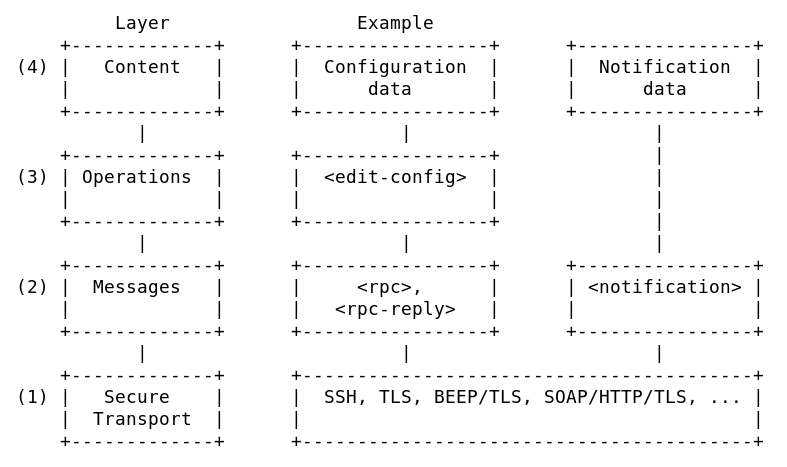
\includegraphics[width=.4\textwidth]{bisdn/netconf}
    \caption{NETCONF protocol layers \cite {CITE - Basebox architecture}}
\end{figure}

\par Data models and operations, covered in detail in the previous section, is related to the Content layer on the image, so this will not be covered in this section. 
\par Configuration of a network device can be complex, and managing separate configurations between device startup and normal operation is a difficult task, but there is occasional need for this capability. NETCONF defines the 
existence of different \textit{datastores} to enable this feature, allowing the network operator to set an initial configuration, used when the device is initialized, and switching to the running datastore when the device is ready
to maintain normal operation. This concept of datastores also enables the creation of a candidate datastore, providing the capability of testing configurations on the network device, checking for any possible errors, while making
sure that there is no impact on the current configuration of the device. After the changes have been tested and validated, a <commit> operation can be used to deploy the new configuration to the running datastore.
\par Another useful feature that is described in the NETCONF protocol, is the possibility of using the rollback-on-error capability. When rolling a new change, and if the system is enabled to support this feature,
NETCONF can detect errors in the changes done to the configurations, and return the system to the previous state that is error free. 
\par The NETCONF API provides several operations to interact with the managed devices to get system information and push new configurations. The set of supported operations in the base NETCONF protocol can be accessed in 
\url{https://tools.ietf.org/html/rfc6241#section-7}. 
\par In regards to the transport layer, NETCONF is able to run on top of several protocols. However, NETCONF requires that a persistent connection is maintained between devices, and this connection should be reliable, and support
transmission failure. In addition, the security should be handled by the transport layer \cite { CITE - https://www.ietf.org/slides/slides-edu-netconf-yang-00.pdf}, providing the guarantee that transactions are done in a 
cryptographically secure channel, between two authenticated hosts. As a results, typical NETCONF implementations are based on SSH or TLS protocols.

\subsection {gRPC}  \label {ssec:grpc}

The basic idea behind the RPC system is defining services by setting the interaction between remote systems, allowing for directly calling objects on remote systems. Based in the client/server communications 
pattern, gRPC allows for interactions between different environments, even implemented with different programming languages, all based on the same data structure. This data structure can be serialized using another modelling 
language, called \textit {protobuf}, which will define the data, which is defined as messages, and the services that contain the RPC calls between systems. Since this system is based on the HTTP2 transport layer, we are able to
use the advantages that this protocol provides us.
\par Despite the serialization language used in gRPC is based on protocol buffers, unlike YANG, there are some projects \footnote {https://github.com/openconfig/goyang} that enable the translation between YANG to protofile,
which allows us to use the data models we chose, only adding one extra step to convert the files.
\par Despite both protocols capability of meeting the requirements that were presented to us, the gRPC framework was chosen due to several reasons:

\begin {itemize}
    \item Both frameworks allow us to use the standardized data models currently proposed by the IETF and OpenConfig
    \item NETCONF trades information as XML encoded information, for both the edit and get config operations; while gRPC allows to handle information in a way that’s native to the language implementation of the client/server
    \item The integration with the existing system was easier: since gRPC has implementations for the languages that the controllers are developed on (i.e. C++/ Python), this framework was easier to implement 
        than NETCONF, which would have required integration with third party tools, or a longer development cycle to make sure that the developed applications would met the requirements
\end {itemize}

\section {Results}



\chapter{Elephant Flow Monitoring} \label{chap:me} 

\section {Testing}

The design of a testing environment must allow for the accurate simulation of the traffic conditions on the real DCNs, and should provide the flexibility to 
understand and change the underlying topologies. There requirements clearly indicate a strong motivation for deploying a testing environment in a virtualised
environment, using tools like \textit{mininet}, which provides a miniature network that can be changed as needed. This testing suite provides a strong 
alternative to deploying these changes in hardware.

\par Despite the developments previously made to the SDN controllers, utilizing these in combination with the virtualised environment poses a challenge, related 
to the implementation of the OpenFlow protocol in the hardware and software switches. Hardware switches that were used for testing in the implementation of
the GUI have a modified version of the OpenFlow tables structure, OFDPA \footnote{OpenFlow Data-Path Abstraction}, and the libraries that make up the 
controller are designed around this. To utilize the controllers, changes to OpenvSwitch would be required, or an alternative would have to be 
discovered, which would limit functionality of the controllers.

\par To solve this issue, and to have a stable controller, that works as intended, for this step we adopt a different controller, and focus on the mechanisms that 
are also present in the hardware controllers. Furthermore, researching other approaches provides ideas that can later be adopted in these. The chosen controller
was Floodlight \footnote { XXX - insert link here}, for it is continuously updated, and provides a REST API for obtaining statistics, setting table rules.

\par These elements compose the testing environment that seen in \ref{fig:test_setup}. To ease the installation of the utilized applications, 
we based these applications on VMs and containers, and the installation files can be found on the following page \url {example.com}.

\pagebreak

\begin{figure} 
    \centering
    \includegraphics[width=0.5\textwidth]{meter_eleph/testing_setup}
    \caption {The high level overview of the testing setup}
    \label{fig:test_setup}
\end{figure} 

\par Figure \ref{fig:test_setup} describes the testing setup designed for testing during this dissertation. This setup provides a close approximation to setups used in the edge layers of data centers, and keeping the
resource consumption of the virtualised network and controller to a minimum. In the diagram, the hosts are shown using the H\textsubscript{X} notation, ranging from 1 to 4, and the switches use the S\textsubscript{X} 
notation. Information about the hosts, like the IP and MAC addresses can also be seen, and the port numbers used are also displayed.

\subsection{Performed tests}

Mininet provides an API to interact with a virtual network and setup tests in a predictable manner. We utilize this API to develop a script that creates the network topology. For traffic generation, however, we require another tool that provides 
specific funcionalities, like control of the packet interval and the packets data size. The tool \textit{hping} is a common tool used for packet generation and port mapping, and its simplicity allows for quickly deploy different tests
against the designed setups.

\par We consider two different test scenarios, the first where we assume no background traffic between the hosts, and the other where every host is communicating with each other. This has the purpose of simulating low traffic intensities in the network,
and verify the behaviour of the designed algorithm in an approximation to real conditions.

\par The utilization of Open vSwitch has, however some drawbacks that should be address when the tests are being designed. Figure \ref{fig:ovs_packet_loss} shows the decrease of 

\begin{figure} 
    \centering
    \includegraphics[width=0.5\textwidth]{}
    \caption {}
    \label{fig:ovs_packet_loss}
\end{figure} 

\section {Algorithm design}

\begin {equation*}
\centering
x_i = 
\begin{bmatrix}
B_{RX}\\
P_{RX}\\
B_{TX}\\
P_{TX}\\
\end{bmatrix}
\end {equation*}

\par $B_{XX}$ and $P_{XX}$ describe to the port statistics obtained from the controller, the byte (B\textsubscript{XX}) and packet (P\textsubscript{XX}) counters, respectively, and the indexes describe if the counters
account for the transmitted or received data in that port.

\par Using the techniques presented in section \ref{subsec:change_detection}, we build algorithm \ref{alg:high_level}. This is a high level view of the steps required to obtain the detection, and in the following sections,
we introduce each step, and provide some clarifications on the design decisions.

\pagebreak

\begin{algorithm}[H]
    \caption{Elephant Detection Algorithm - High Level} \label{alg:high_level}
    \begin{algorithmic}[1]
        \Procedure {Elephant Flow Detection}{}
            \State Initialization
            \State Query controller
            \Loop
                \State Error calculation
                \State Prediction
                \State Detection
                \If {Detection}
                    \State Raise Alarm
                \EndIf
            \EndLoop
        \EndProcedure 
        \State \Return Alarm Times
    \end{algorithmic}
\end{algorithm}

\subsection{Initialization}

The initialization step of the algorithm is a crucial step for obtaining correct results in the algorithm. This step allows for the correct initialization of the model parameters, including the trend component, and to provide a 
baseline for the expected traffic on the network. Due to these factors, it is assumed that no traffic abnormalities exist during this stage, but a longer period for initialization can account for short bursts of higher traffic.

\begin{algorithm}[H]
    \caption{Elephant Detection Algorithm - Initialization} \label{alg:high_level}
    \begin{algorithmic}[1]
        \Procedure {Initialization}{}
            \State initialization period = 30s
            \While {t <= initialization period}
                \State x = Query controller
                \State initialization measures += x
                \State Determine prediction
            \EndWhile
            \State Linear Regression (initialization measures)
        \State \Return Linear regression coefficient
    \end{algorithmic}
\end{algorithm}

\par Detrending the data using the linear regression function comes from the fact that on the end of the initialization period, plotting the received bytes results in figure \ref{fig:init_plot}.

% Display initial graph of Received Bytes
\begin{figure} 
    \centering
    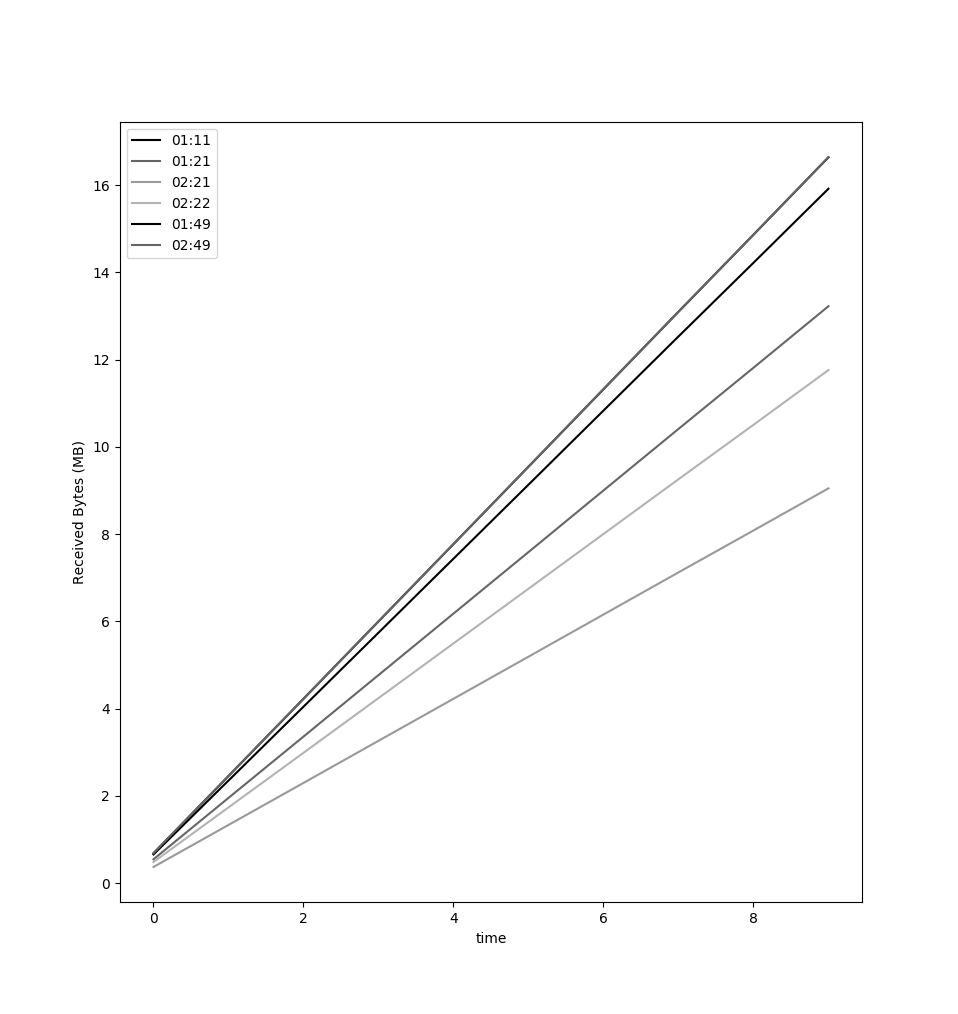
\includegraphics[width=0.5\textwidth]{meter_eleph/init_period_lin}
    \caption {Plotting the initial measurements of B\textsubscript{RX}}
    \label{fig:init_plot}
\end{figure} 

\subsection{Error calculation}

\subsection{Prediction}

\subsection{Calculation}


\section {Tests}
\section {Results}


%\chapter{Testing setup and environment} \label{chap:me} %% chapter 3

\section {Introduction}

In the next sections, we discuss and evaluate the environment used for generating and evaluating the test results. The testing environment aims to replicate the lower layers of the data center topologies, as demonstrated in 
figure \ref{nm/fattree}, due to faster response of mitigation of the elephant flows, generating less impact in the network, as seen in \cite { CITE - http://ieeexplore.ieee.org/document/7366826/}, while also reducing the 
resource consumption of physical memory and processing power associated with creating very large virtualized networks. 

\section {Time series database}
\section {Switches}
\subsection {OF-DPA}
\subsection {Mininet}
\section {OpenFlow controllers}
\section {Testing Methodologies}
\subsection {Traffic generation}
\subsection {Traffic control}

%\chapter{Elephant Flow Monitoring} \label{chap:me} 

\section {Testing}

The design of a testing environment must allow for the accurate simulation of the traffic conditions on the real DCNs, and should provide the flexibility to 
understand and change the underlying topologies. There requirements clearly indicate a strong motivation for deploying a testing environment in a virtualised
environment, using tools like \textit{mininet}, which provides a miniature network that can be changed as needed. This testing suite provides a strong 
alternative to deploying these changes in hardware.

\par Despite the developments previously made to the SDN controllers, utilizing these in combination with the virtualised environment poses a challenge, related 
to the implementation of the OpenFlow protocol in the hardware and software switches. Hardware switches that were used for testing in the implementation of
the GUI have a modified version of the OpenFlow tables structure, OFDPA \footnote{OpenFlow Data-Path Abstraction}, and the libraries that make up the 
controller are designed around this. To utilize the controllers, changes to OpenvSwitch would be required, or an alternative would have to be 
discovered, which would limit functionality of the controllers.

\par To solve this issue, and to have a stable controller, that works as intended, for this step we adopt a different controller, and focus on the mechanisms that 
are also present in the hardware controllers. Furthermore, researching other approaches provides ideas that can later be adopted in these. The chosen controller
was Floodlight \footnote { XXX - insert link here}, for it is continuously updated, and provides a REST API for obtaining statistics, setting table rules.

\par These elements compose the testing environment that seen in \ref{fig:test_setup}. To ease the installation of the utilized applications, 
we based these applications on VMs and containers, and the installation files can be found on the following page \url {example.com}.

\pagebreak

\begin{figure} 
    \centering
    \includegraphics[width=0.5\textwidth]{meter_eleph/testing_setup}
    \caption {The high level overview of the testing setup}
    \label{fig:test_setup}
\end{figure} 

\par Figure \ref{fig:test_setup} describes the testing setup designed for testing during this dissertation. This setup provides a close approximation to setups used in the edge layers of data centers, and keeping the
resource consumption of the virtualised network and controller to a minimum. In the diagram, the hosts are shown using the H\textsubscript{X} notation, ranging from 1 to 4, and the switches use the S\textsubscript{X} 
notation. Information about the hosts, like the IP and MAC addresses can also be seen, and the port numbers used are also displayed.

\subsection{Performed tests}

Mininet provides an API to interact with a virtual network and setup tests in a predictable manner. We utilize this API to develop a script that creates the network topology. For traffic generation, however, we require another tool that provides 
specific funcionalities, like control of the packet interval and the packets data size. The tool \textit{hping} is a common tool used for packet generation and port mapping, and its simplicity allows for quickly deploy different tests
against the designed setups.

\par We consider two different test scenarios, the first where we assume no background traffic between the hosts, and the other where every host is communicating with each other. This has the purpose of simulating low traffic intensities in the network,
and verify the behaviour of the designed algorithm in an approximation to real conditions.

\par The utilization of Open vSwitch has, however some drawbacks that should be address when the tests are being designed. Figure \ref{fig:ovs_packet_loss} shows the decrease of 

\begin{figure} 
    \centering
    \includegraphics[width=0.5\textwidth]{}
    \caption {}
    \label{fig:ovs_packet_loss}
\end{figure} 

\section {Algorithm design}

\begin {equation*}
\centering
x_i = 
\begin{bmatrix}
B_{RX}\\
P_{RX}\\
B_{TX}\\
P_{TX}\\
\end{bmatrix}
\end {equation*}

\par $B_{XX}$ and $P_{XX}$ describe to the port statistics obtained from the controller, the byte (B\textsubscript{XX}) and packet (P\textsubscript{XX}) counters, respectively, and the indexes describe if the counters
account for the transmitted or received data in that port.

\par Using the techniques presented in section \ref{subsec:change_detection}, we build algorithm \ref{alg:high_level}. This is a high level view of the steps required to obtain the detection, and in the following sections,
we introduce each step, and provide some clarifications on the design decisions.

\pagebreak

\begin{algorithm}[H]
    \caption{Elephant Detection Algorithm - High Level} \label{alg:high_level}
    \begin{algorithmic}[1]
        \Procedure {Elephant Flow Detection}{}
            \State Initialization
            \State Query controller
            \Loop
                \State Error calculation
                \State Prediction
                \State Detection
                \If {Detection}
                    \State Raise Alarm
                \EndIf
            \EndLoop
        \EndProcedure 
        \State \Return Alarm Times
    \end{algorithmic}
\end{algorithm}

\subsection{Initialization}

The initialization step of the algorithm is a crucial step for obtaining correct results in the algorithm. This step allows for the correct initialization of the model parameters, including the trend component, and to provide a 
baseline for the expected traffic on the network. Due to these factors, it is assumed that no traffic abnormalities exist during this stage, but a longer period for initialization can account for short bursts of higher traffic.

\begin{algorithm}[H]
    \caption{Elephant Detection Algorithm - Initialization} \label{alg:high_level}
    \begin{algorithmic}[1]
        \Procedure {Initialization}{}
            \State initialization period = 30s
            \While {t <= initialization period}
                \State x = Query controller
                \State initialization measures += x
                \State Determine prediction
            \EndWhile
            \State Linear Regression (initialization measures)
        \State \Return Linear regression coefficient
    \end{algorithmic}
\end{algorithm}

\par Detrending the data using the linear regression function comes from the fact that on the end of the initialization period, plotting the received bytes results in figure \ref{fig:init_plot}.

% Display initial graph of Received Bytes
\begin{figure} 
    \centering
    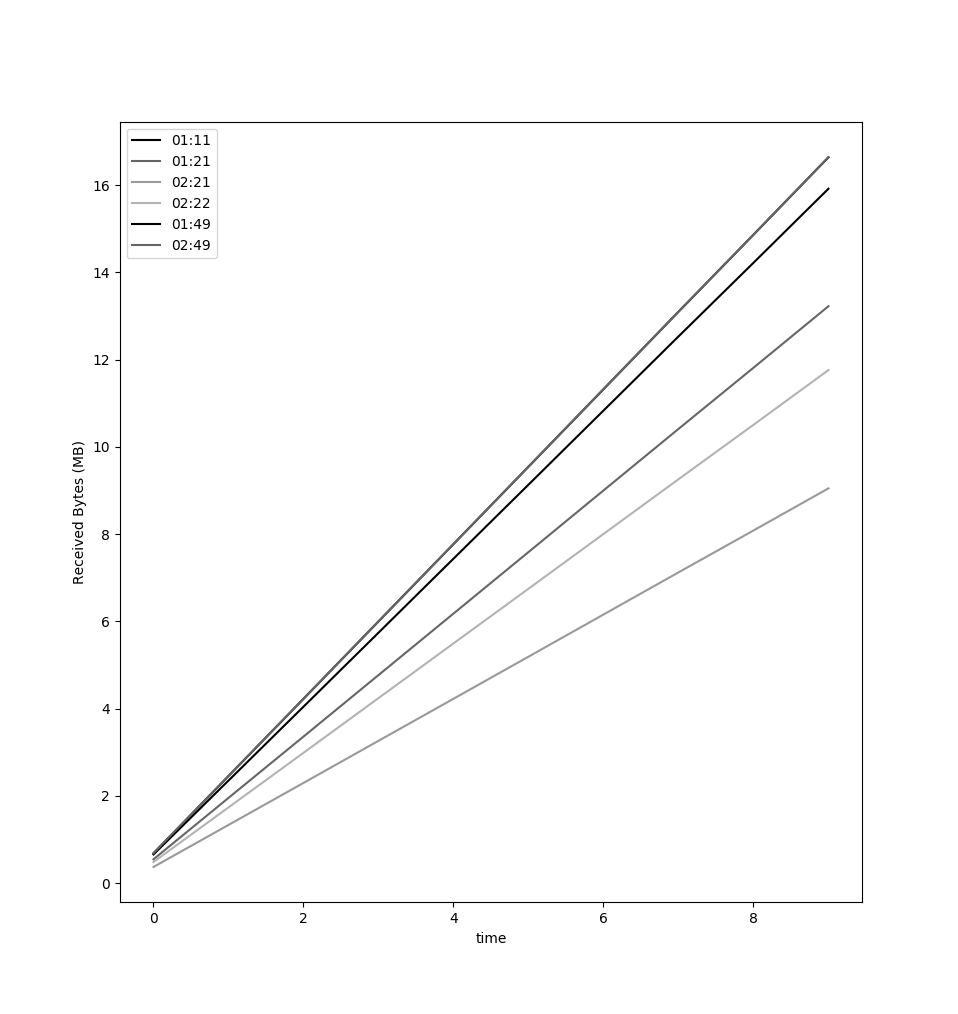
\includegraphics[width=0.5\textwidth]{meter_eleph/init_period_lin}
    \caption {Plotting the initial measurements of B\textsubscript{RX}}
    \label{fig:init_plot}
\end{figure} 

\subsection{Error calculation}

\subsection{Prediction}

\subsection{Calculation}


\section {Tests}
\section {Results}


%\chapter{Conclusion}

\section{Summary of Results}

The main objective for this thesis was building a management system that would integrate with a pre-existing Software-Defined Network controller, exposing information
for network operators to manage and configure their networking infrastructure. With these requirements, we have proposed a management environment that extends a
previously existing system, by adding an interface to baseboxd and CAWR, two SDN controllers composing the Basebox environment, allowing further developments in the 
field of Traffic Engineering with these systems.  Integrating this system, we have designed a Graphical User Interface for interaction with the users, allowing for
simple visualisation of the network's physical topology, and the display of interfaces' statistics, like the packets and bytes received and sent, or the number of 
errors. 

\par We have also proposed an algorithm that allows for monitoring traffic changes in ports, in order to detect elephant flows in the network. Despite not having
used the Basebox system for testing this algorithm, due to differences in the testing environment, we believe that the same algorithm can be used for large flow 
detection in the Basebox stack, by changing the interface for obtaining statistics. We have shown that a simple method can be employed by operators to monitor the
state of their network, and rely on this algorithm to provide them with alarms of port changes.

\section{Future Work}

Despite our conclusion that the main objectives of the thesis were achieved, the large scope of themes that this topic encompasses means that not everything could be 
successfully covered. As for more immediate concerns, the next steps in guaranteeing a stable product would be the expansion  of the GUI to report and configure 
VLANs in each port that is monitored; and support layer 3 functionality, such as visualising next hop neighbours, routing tables, etc. In regards to longer term
goals, continuing the work on monitoring not only the port change, but the actual flow that contributes to the largest changes in ports. This could be expanded 
into a system that analyses the services and applications that contribute the most to the traffic volumes in the network, which can then be further optimized by 
reporting the periodicity of the largest traffic volumes. The aspect of providing a system that can discriminate the traffic by transport protocol is also an 
interesting research topic for improving Quality of Service in Software-Defined Networks.


%% comment next 2 commands if numbered appendices are not used
%\appendix
%\chapter{Appendix}

\section{GUI icons mapping}
\begin{table}[H]
    \centering
    \caption{GUI icons and their meaning}
    \label{tab:gui-mapping}
    \begin{tabular}{l | l}
        \centering
            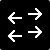
\includegraphics[width=.05\textwidth]{bisdn/switch}
        & switch     & \\ \hline 
            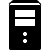
\includegraphics[width=.05\textwidth]{bisdn/host}
        & host     & \\ \hline 
        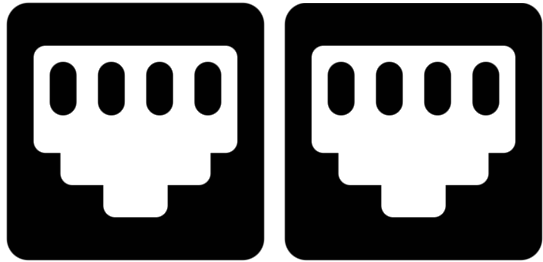
\includegraphics[width=.05\textwidth]{bisdn/bond}
        & port     & \\
   \end{tabular}
\end{table}


%%----------------------------------------
%% Final materials
%%----------------------------------------

%% Bibliography
%% Comment the next command if BibTeX file not used
%% bibliography is in ``myrefs.bib''

\PrintBib{Thesus}

%% Index
%% Uncomment next command if index is required
%% don't forget to run ``makeindex thesis'' command
%\PrintIndex

\end{document}
